% Soutenance de mémoire — version LaTeX (Beamer), 15 diapositives, 12 minutes.
% Compilation : pdflatex (deux passes). Les figures proviennent de ./images/ (copiées de latex/images/).
\documentclass[10pt,aspectratio=169]{beamer}

\usepackage[T1]{fontenc}
\usepackage[utf8]{inputenc}
\usepackage{lmodern}
\usepackage[french]{babel}
\usepackage{graphicx}
\usepackage{booktabs}
\usepackage{multicol}

\definecolor{swarmnavy}{HTML}{10243B}
\definecolor{swarmtext}{HTML}{16243A}
\definecolor{swarmmuted}{HTML}{5B6B80}
\definecolor{swarmblue}{HTML}{1F4E79}
\definecolor{swarmgold}{HTML}{E3B341}
\definecolor{swarmcard}{HTML}{F1F4F8}
\definecolor{swarmline}{HTML}{D4DCE7}

\usetheme{default}
\setbeamercolor{normal text}{fg=swarmtext, bg=white}
\setbeamercolor{structure}{fg=swarmblue}
\setbeamercolor{title}{fg=swarmtext}
\setbeamercolor{frametitle}{fg=swarmtext, bg=white}
\setbeamercolor{block title}{fg=white, bg=swarmblue}
\setbeamercolor{block body}{fg=swarmtext, bg=swarmcard}
\setbeamercolor{block title example}{fg=swarmtext, bg=swarmgold}
\setbeamercolor{itemize item}{fg=swarmblue}
\setbeamercolor{item}{fg=swarmblue}
\setbeamertemplate{itemize item}[triangle]
\setbeamertemplate{navigation symbols}{}
\setbeamertemplate{frametitle}{%
  \nointerlineskip
  \begin{beamercolorbox}[wd=\paperwidth,leftskip=0.6cm,ht=1.05cm,dp=0.35cm]{frametitle}%
    \usebeamerfont{frametitle}\usebeamercolor[fg]{frametitle}\insertframetitle%
  \end{beamercolorbox}%
  \vspace{-0.55cm}%
  {\color{swarmgold}\rule{0.9cm}{1.2pt}}\par
}
\setbeamertemplate{footline}{%
  \leavevmode\hbox{}\hfill\usebeamerfont{footline}\textcolor{swarmmuted}{\insertframenumber\ /\inserttotalframenumber}\hspace{0.6cm}\vspace{0.25cm}%
}
\setlength{\parskip}{0.35em}

\title{Contrôle décentralisé d'un essaim de robots par réseaux de neurones sur graphe}
\subtitle{Formation de contours géométriques et symboliques par apprentissage différentiable, exécution locale et passage à l'échelle}
\author{Laurent MWANAMPUTU LABEYA}
\institute{Université de Kinshasa (UNIKIN) \par Faculté des Sciences et Technologies \par Option : Intelligence artificielle et Sciences des données}
\date{Soutenance de mémoire, Master --- Année académique 2025--2026 \\[0.2em] Directeur : Prof. Dr Selain KASEREKA KABUNGA}

\begin{document}

% 1 --- Couverture
{
\setbeamercolor{background canvas}{bg=swarmnavy}
\setbeamercolor{normal text}{fg=white}
\begin{frame}[plain]
  \vspace*{-0.1cm}
  {\color{swarmgold}\footnotesize\bfseries SOUTENANCE DE MÉMOIRE --- MASTER, 2026\par}
  \vspace{0.5cm}
  {\usebeamerfont{title}\color{white}\LARGE\bfseries Contrôle décentralisé d'un essaim de robots\\[0.25em] par réseaux de neurones sur graphe\par}
  \vspace{0.4cm}
  {\color{swarmgold}\rule{3cm}{1.6pt}\par}
  \vspace{0.4cm}
  {\color{white}\normalsize\itshape Formation de contours géométriques et symboliques par apprentissage différentiable, exécution locale et passage à l'échelle\par}
  \vfill
  \begin{columns}[T]
    \begin{column}{0.68\textwidth}
      {\color{white}\textbf{Laurent MWANAMPUTU LABEYA}\\[0.15em]
      \color{swarmgold}\rule{0.9cm}{1.2pt}\\[0.35em]
      \small Directeur : Prof. Dr Selain KASEREKA KABUNGA\\
      \small Faculté des Sciences et Technologies, UNIKIN\par}
    \end{column}
    \begin{column}{0.32\textwidth}
      \raggedleft
      
\includegraphics[height=2.0cm,keepaspectratio]{images/logo_unikin.png}\par
      {\color{white}\scriptsize 12 minutes · 15 diapositives\par}
    \end{column}
  \end{columns}
\end{frame}
}

% 2 --- Problématique
\begin{frame}{Deux familles de contrôleurs, une seule question}
  \begin{columns}[T]
    \begin{column}{0.55\textwidth}
      \textbf{Règle écrite} --- attraction, répulsion, alignement : interprétable, mais sans géométrie précise de cible.\par
      \textbf{Règle apprise} --- un GNN reçoit les voisins et la consigne de forme : davantage de paramètres, de coût de calcul, et une robustesse à vérifier.\par
      \vspace{0.4cm}
      \begin{block}{Question}
        Dans quelles conditions une règle apprise, exécutée localement, peut-elle être une alternative raisonnable à une règle manuelle ?
      \end{block}
    \end{column}
    \begin{column}{0.45\textwidth}
      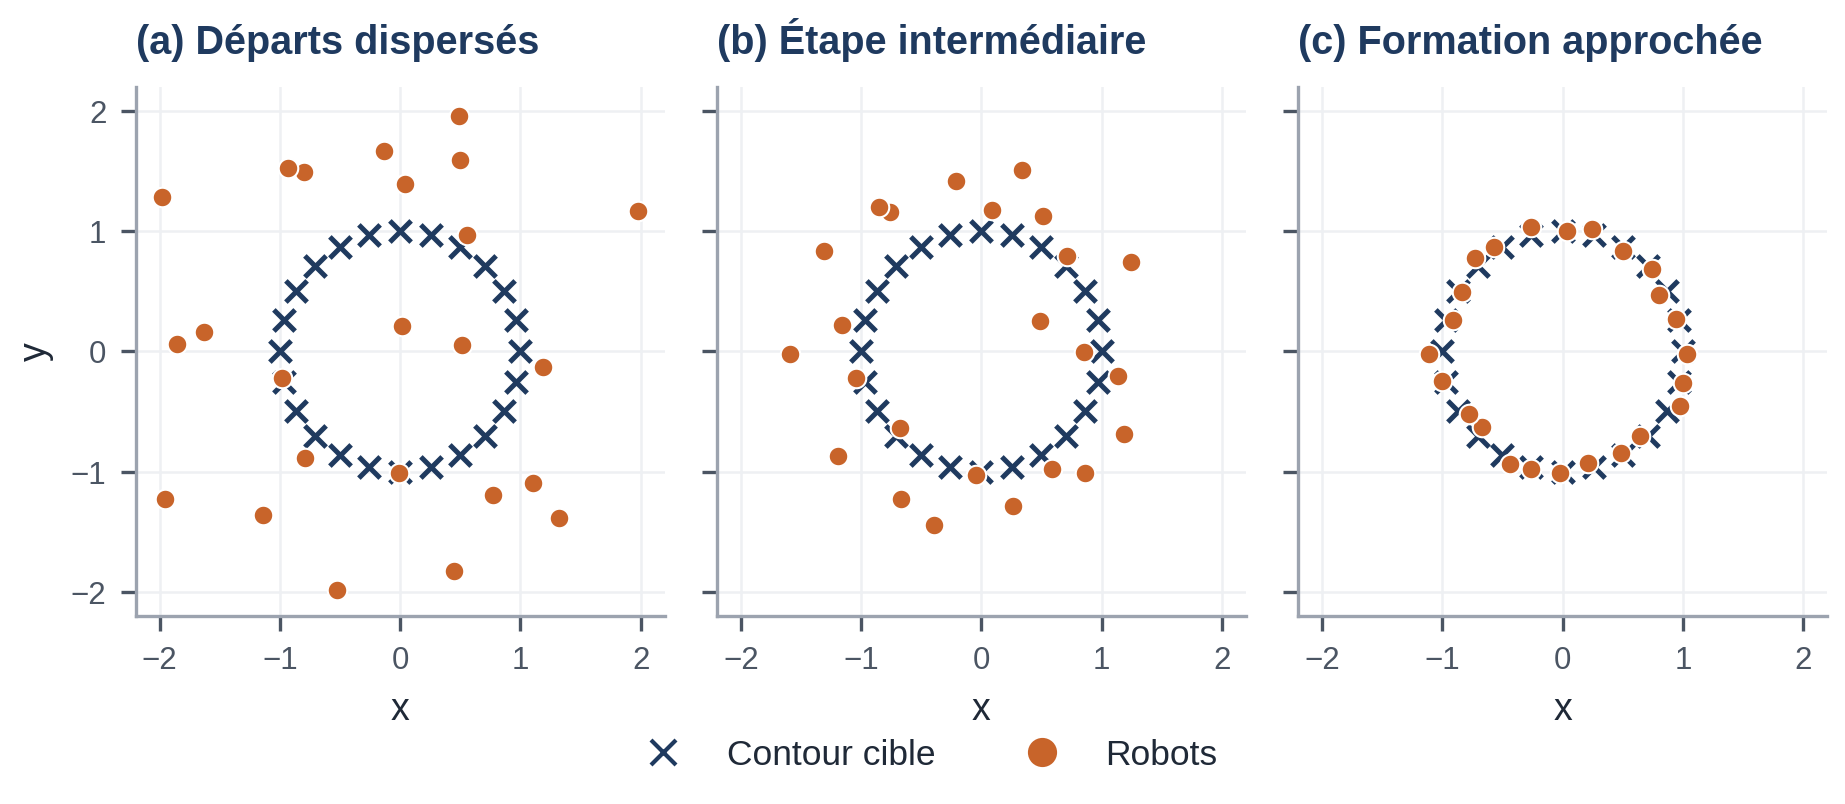
\includegraphics[width=\textwidth,keepaspectratio]{images/formation_principle.png}\par
      \vspace{0.2cm}
      {\footnotesize\itshape\color{swarmmuted} Les robots convergent vers un nuage de points, sans affectation permanente robot--point.\par}
    \end{column}
  \end{columns}
\end{frame}

% 3 --- Travaux connexes
\begin{frame}{Trois travaux, un angle mort partagé}
  \begin{multicols}{3}
    \textbf{\color{swarmblue}Hsieh, Kumar \& Chaimowicz --- 2008}\\[0.2em]
    Générer des formes par règles locales. L'information géométrique accessible localement est déterminante.\par
    {\footnotesize\color{swarmmuted}\textbf{Manque :} aucune comparaison avec une politique apprise à information égale.\par}
    \columnbreak
    \textbf{\color{swarmblue}Tolstaya et al. --- 2020}\\[0.2em]
    Un GNN entraîné pour des tâches d'essaim, exécuté localement sur un graphe de communication mobile.\par
    {\footnotesize\color{swarmmuted}\textbf{Manque :} rien sur la lisibilité de lettres, de chiffres ou de nombres.\par}
    \columnbreak
    \textbf{\color{swarmblue}Jiang, Huang \& Guo --- 2023}\\[0.2em]
    Formation triangulaire entraînée avec 5 robots, testée de 4 à 9 ; le LiDAR fournit des cartes locales.\par
    {\footnotesize\color{swarmmuted}\textbf{Manque :} perception différente, l'écart ne revient pas à la seule architecture.\par}
  \end{multicols}
  \vspace{0.3cm}
  \begin{beamercolorbox}[wd=\textwidth,rounded=false,leftskip=0.4cm,dp=1.4em]{block body}
    Comparer seulement à information de consigne comparable : sinon l'écart mesure l'information reçue, pas le contrôleur.
  \end{beamercolorbox}
\end{frame}

% 4 --- Modèle
\begin{frame}{Un essaim, un graphe reconstruit à chaque pas}
  \begin{columns}[T]
    \begin{column}{0.52\textwidth}
      \begin{itemize}
        \item $N$ robots dans une arène de $4\times4$ ; pas de temps $0{,}1$ ; vitesse bornée par $v_{\max}=1$.
        \item Deux robots communiquent si leur distance reste sous la portée $r_c=1{,}5$.
        \item Le nombre et l'ordre des voisins varient : l'agrégation doit être symétrique.
        \item Chaque robot ne commande que sa propre vitesse.
        \item Aucune affectation globale robot--point pendant l'exécution.
      \end{itemize}
      \vspace{0.2cm}
      {\footnotesize\color{swarmmuted}\textbf{Hypothèses fortes, assumées :} repère commun, positions exactes, échanges sans délai ni perte.\par}
    \end{column}
    \begin{column}{0.48\textwidth}
      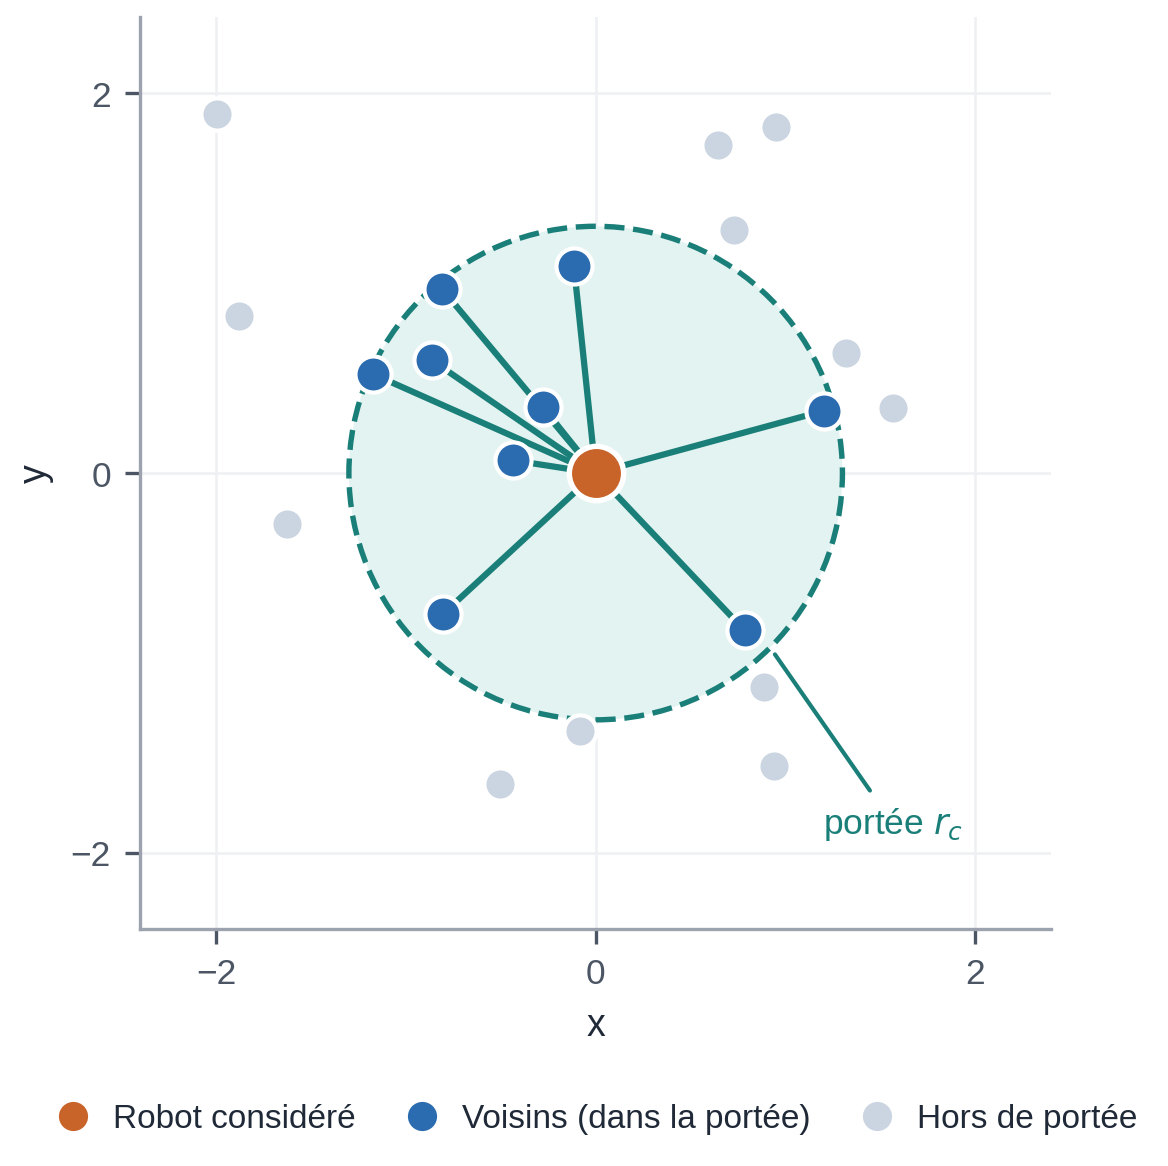
\includegraphics[width=0.92\textwidth,keepaspectratio]{images/swarm_communication_graph.png}\par
      \vspace{0.15cm}
      {\footnotesize\itshape\color{swarmmuted} Graphe de communication à portée disque : les arêtes dépendent seulement des positions.\par}
    \end{column}
  \end{columns}
\end{frame}

% 5 --- Données
\begin{frame}{64 formes, trois résolutions, un découpage figé}
  \begin{itemize}
    \item 64 identifiants : 7 géométries, 10 chiffres, 26 lettres, 21 nombres.
    \item Rendu sur grille $128\times128$, échantillonnage par point le plus éloigné : 20, 40 ou 50 pixels distincts. Jamais de duplication pour atteindre le quota.
    \item Recentrage sur le centroïde, puis normalisation à rayon maximal $R=1$.
    \item Découpage fixe entraînement / validation / test --- le test ne sert ni au réglage ni au choix du modèle.
  \end{itemize}
  \vspace{0.2cm}
  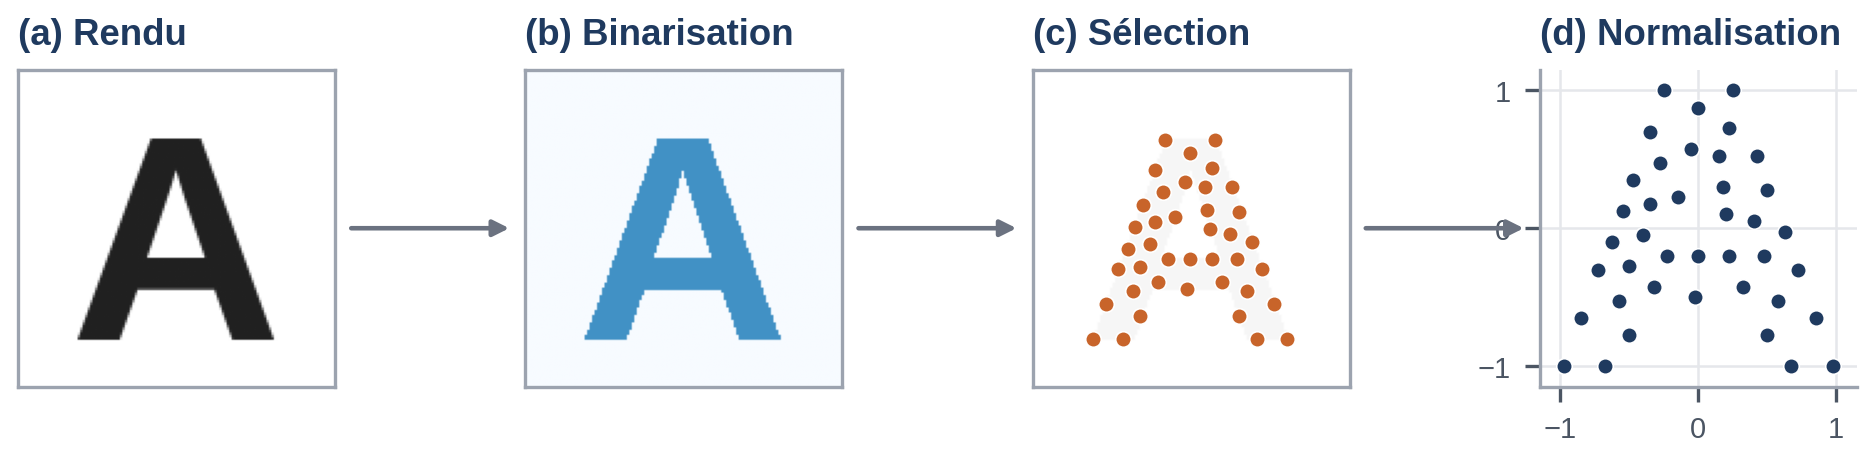
\includegraphics[width=0.86\textwidth,keepaspectratio]{images/target_preparation_pipeline.png}\par
  \vspace{0.1cm}
  {\footnotesize\itshape\color{swarmmuted} Préparation d'une cible : rendu, binarisation, sélection de points, normalisation. L'échelle commune rend les distances sans dimension ; elle n'égalise pas la difficulté des formes.\par}
\end{frame}

% 6 --- Contrôleur
\begin{frame}{Un seul réseau partagé, exécuté localement}
  \begin{itemize}\footnotesize
    \item \textbf{Observation :} vitesse précédente + représentation apprise de l'identifiant (16 composantes) +, en variante géométrique, direction unitaire vers le point cible le plus proche.
    \item \textbf{Encodage :} affine + ReLU (64), puis deux tours de messages agrégés par moyenne ; un seul jeu de poids pour tous les robots.
    \item \textbf{Décodeur borné :} résidu directionnel, tangente hyperbolique, puis projection radiale sous $v_{\max}$.
  \end{itemize}
  \vspace{0.1cm}
  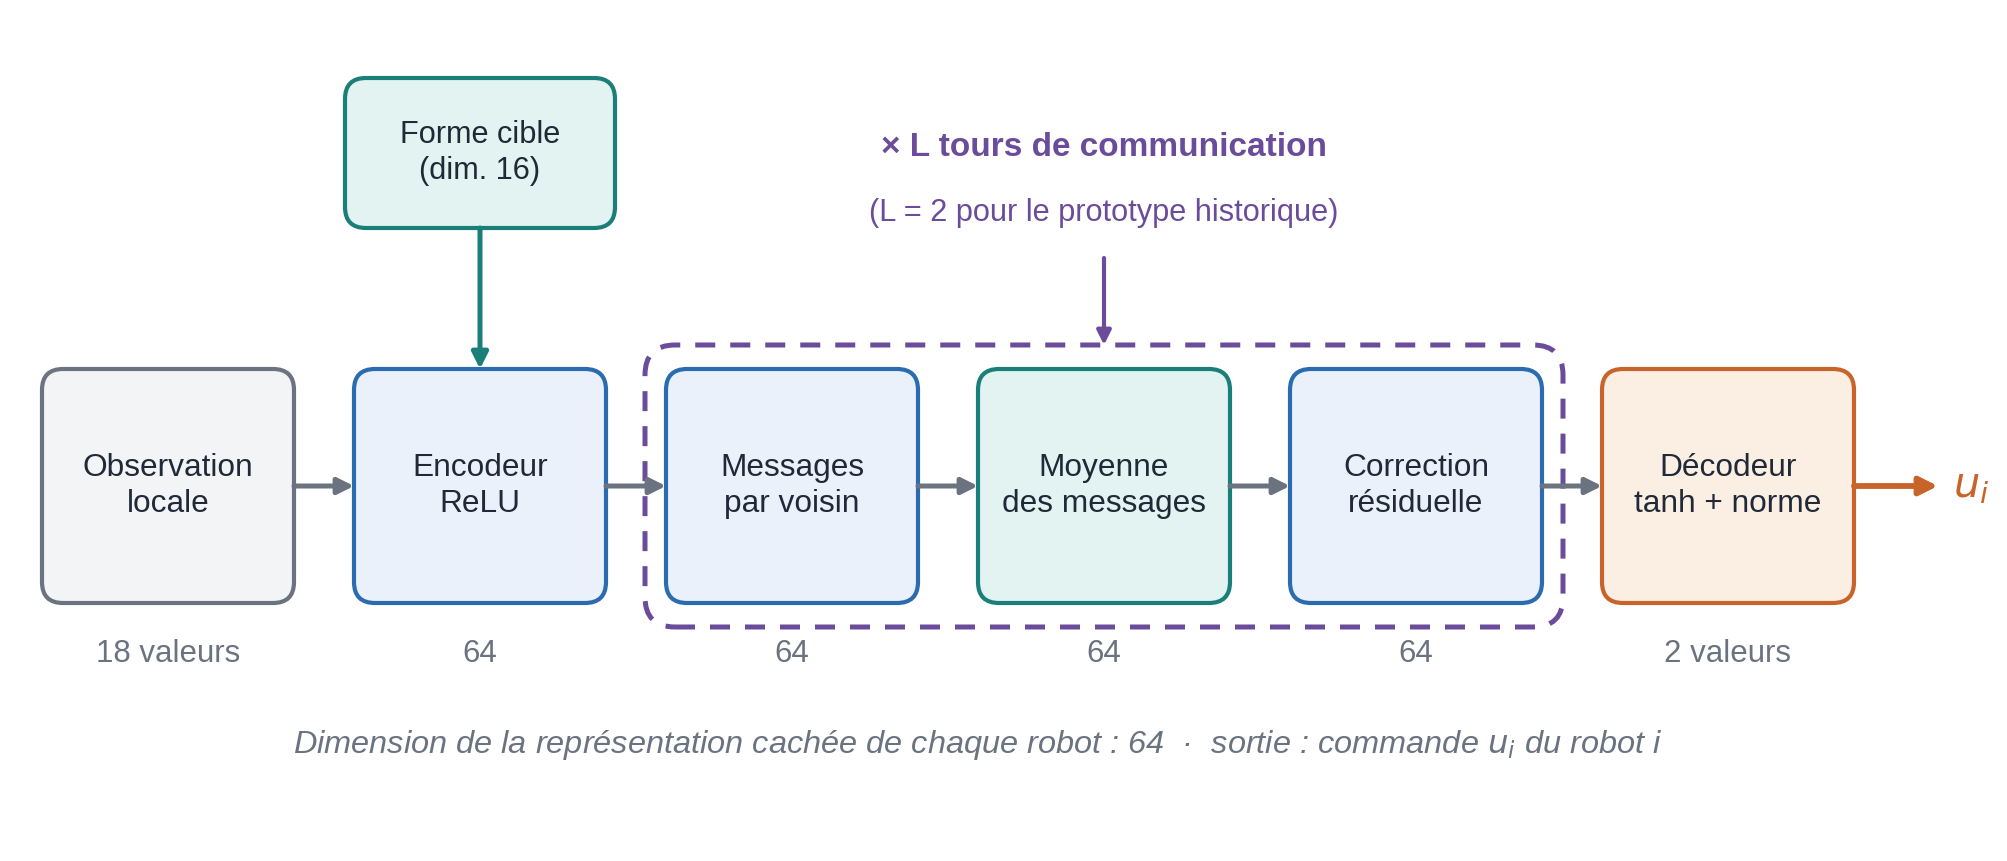
\includegraphics[width=0.74\textwidth,keepaspectratio]{images/gnn_current_architecture.png}\par
  \vspace{0.05cm}
  {\footnotesize\itshape\color{swarmmuted} Architecture de l'implémentation actuelle : observation, encodage, messages, décodage.\par}
\end{frame}

% 7 --- Agrégation
\begin{frame}{L'agrégation par moyenne : sobre, et assumée comme telle}
  \begin{columns}[T]
    \begin{column}{0.5\textwidth}
      \begin{itemize}
        \item Invariance aux permutations exigée par le voisinage variable : la moyenne la satisfait (Zaheer et al., 2017).
        \item Contrairement à une somme non normalisée, elle évite que l'échelle croisse avec le nombre de voisins.
        \item Elle n'a pas pour autant toute la capacité de représentation d'une somme ; l'attention ajoute paramètres et coût.
        \item \textbf{Limite explicite :} un voisin aberrant pèse un poids uniforme, sans filtre.
      \end{itemize}
    \end{column}
    \begin{column}{0.5\textwidth}
      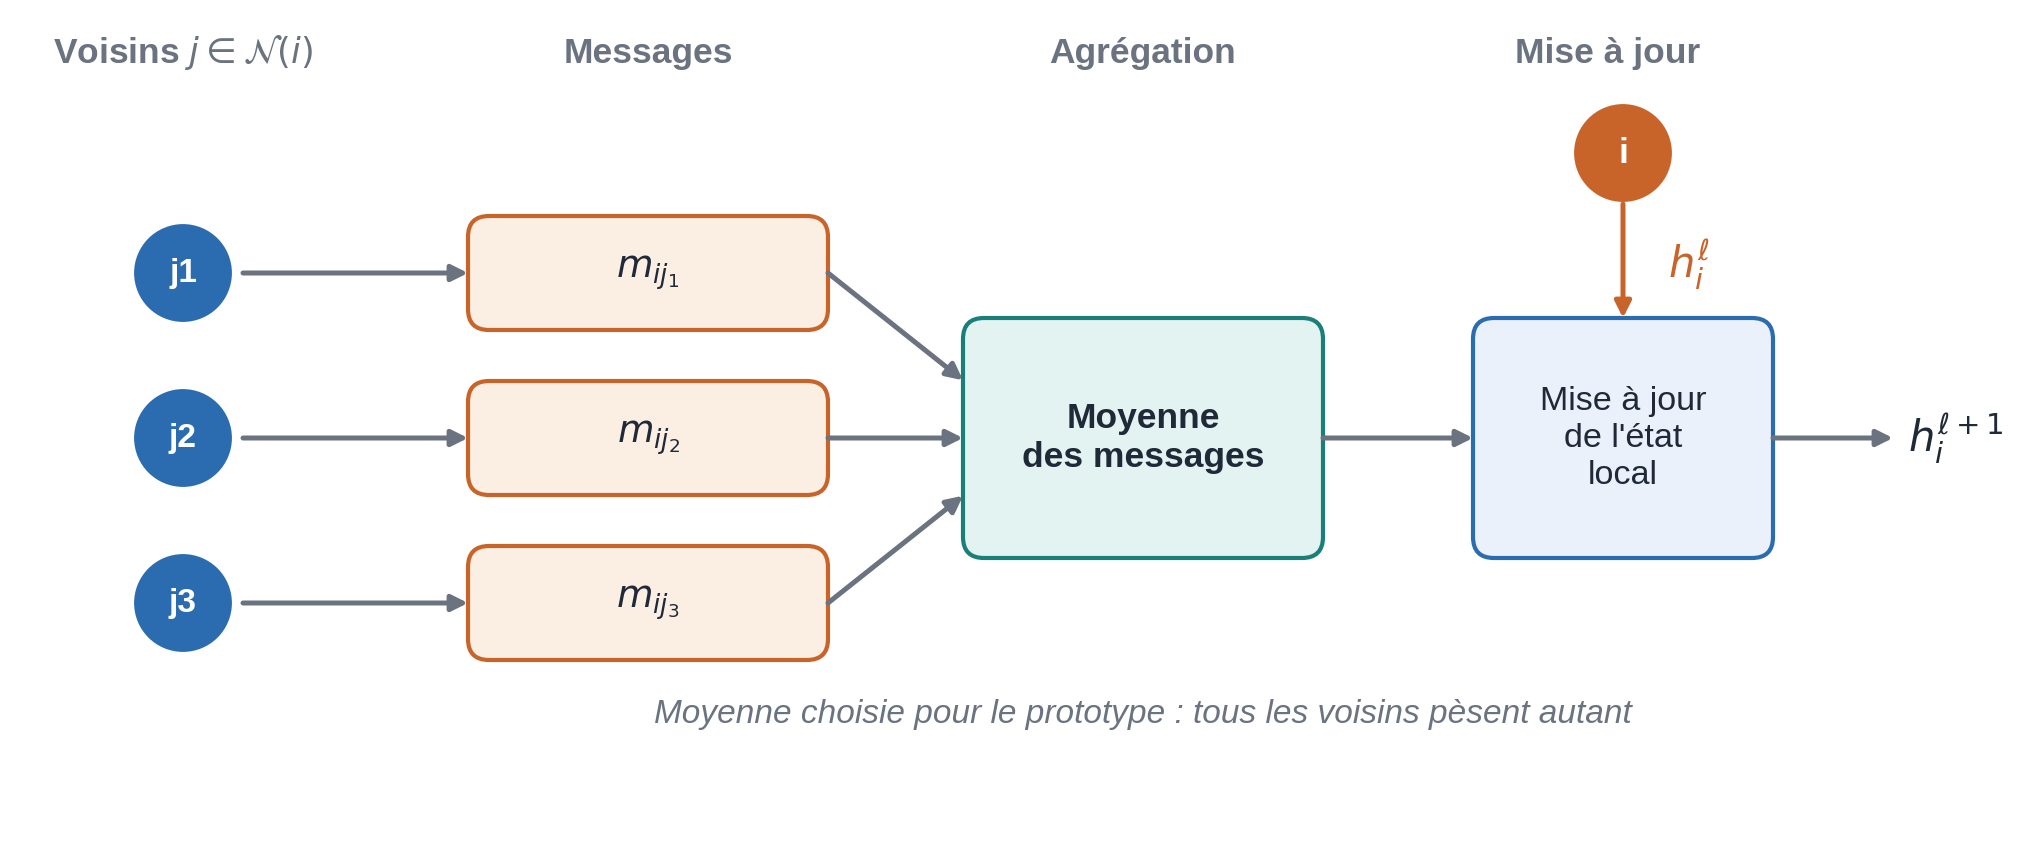
\includegraphics[width=\textwidth,keepaspectratio]{images/message_aggregation.png}\par
      \vspace{0.15cm}
      {\footnotesize\itshape\color{swarmmuted} Somme, moyenne, max : la moyenne retire le facteur de degré, sans garantir la qualité de formation.\par}
    \end{column}
  \end{columns}
\end{frame}

% 8 --- Fonction de coût
\begin{frame}{Une perte, quatre objectifs distincts}
  \begin{columns}[T]
    \begin{column}{0.5\textwidth}
      \begin{itemize}\footnotesize
        \item Chamfer non carrée, normalisée par le rayon $R$ de la cible.
        \item Un sens mesure la proximité des robots au contour, l'autre la couverture de la cible.
        \item Moyenne sur les dix derniers états de la trajectoire, pas seulement l'état final.
        \item Les dix premiers états sont exclus des collisions : le chevauchement initial ne vient d'aucune commande.
        \item Aucun effet causal d'une composante n'est établi sans ablation.
      \end{itemize}
      \vspace{0.1cm}
      \begin{tabular}{@{}lrl@{}}
        \toprule
        forme & \textbf{1,0} & proximité \\
        couverture & \textbf{1,0} & contour complet \\
        collisions & \textbf{0,5} & pénalité paires \\
        mouvement & \textbf{0,02} & régularité \\
        \bottomrule
      \end{tabular}
    \end{column}
    \begin{column}{0.5\textwidth}
      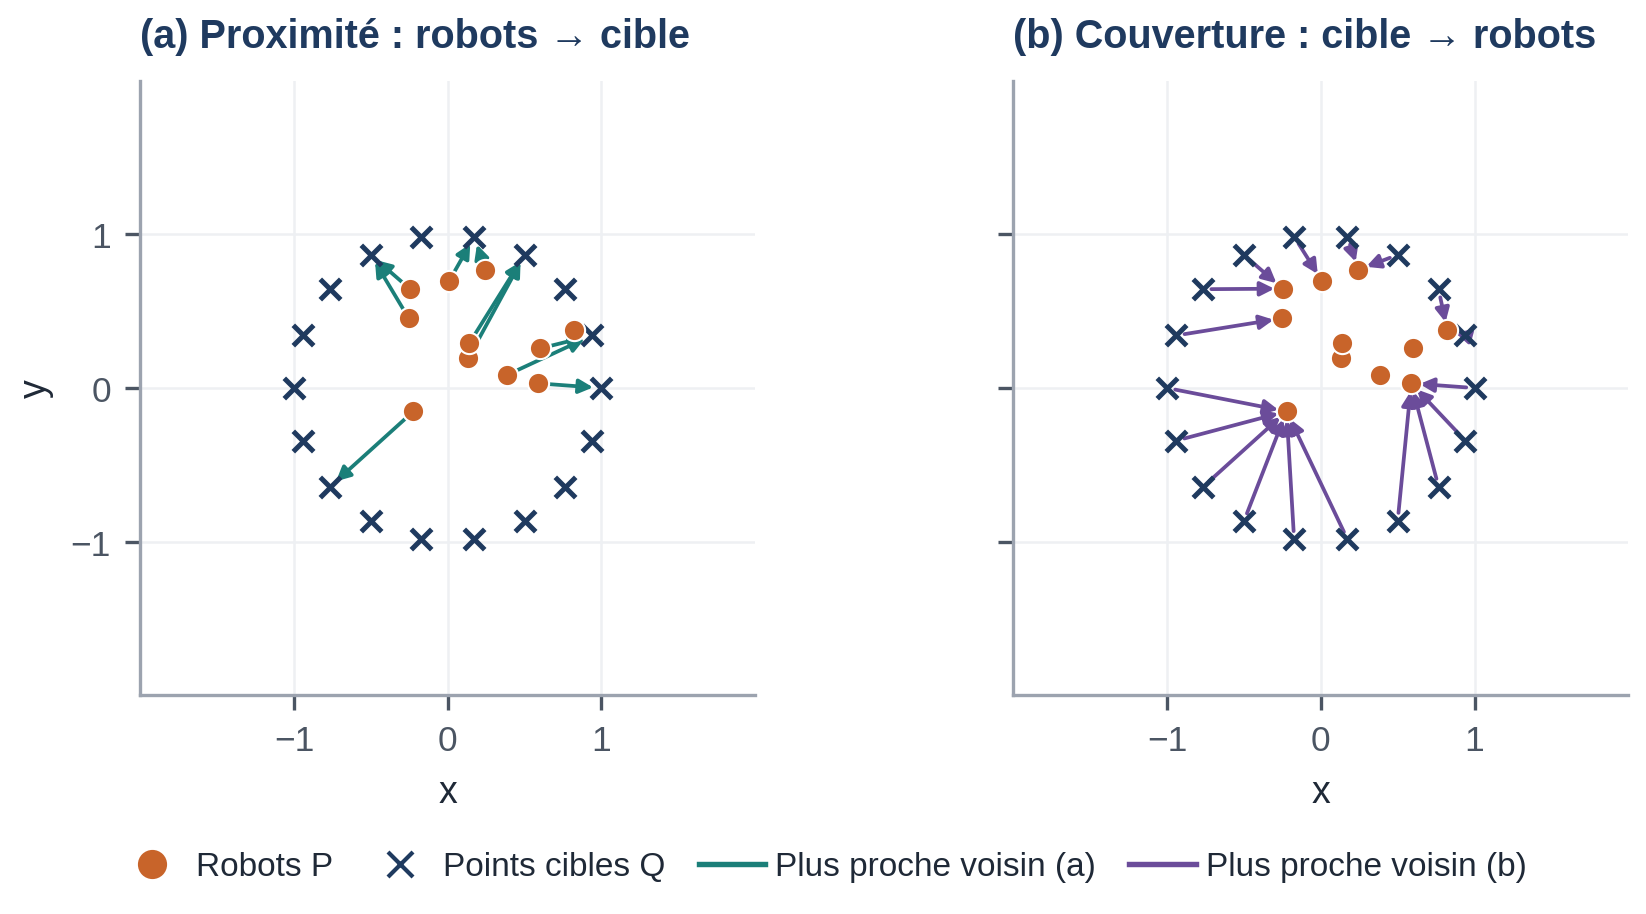
\includegraphics[width=\textwidth,keepaspectratio]{images/shape_loss_geometry.png}\par
      \vspace{0.15cm}
      {\footnotesize\itshape\color{swarmmuted} Deux sens de la comparaison entre ensembles, sans affectation bijective. Un amas peut rester proche de la cible en laissant une partie du contour découvert.\par}
    \end{column}
  \end{columns}
\end{frame}

% 9 --- Apprentissage
\begin{frame}{Gradient direct à travers la simulation}
  \begin{itemize}\footnotesize
    \item Pas d'expert à imiter, pas de récompense estimée par échantillonnage : le signal vient d'une perte de forme calculée en fin d'épisode.
    \item La politique est entraînée dans l'épisode qu'elle produit elle-même---ce qui évite le décalage propre à l'imitation.
    \item Meilleur état sélectionné sur la validation, jamais sur la dernière perte d'entraînement ; le graphe de voisinage et le point le plus proche sont discrets : la simulation est différentiable \emph{par morceaux}.
  \end{itemize}
  \vspace{0.05cm}
  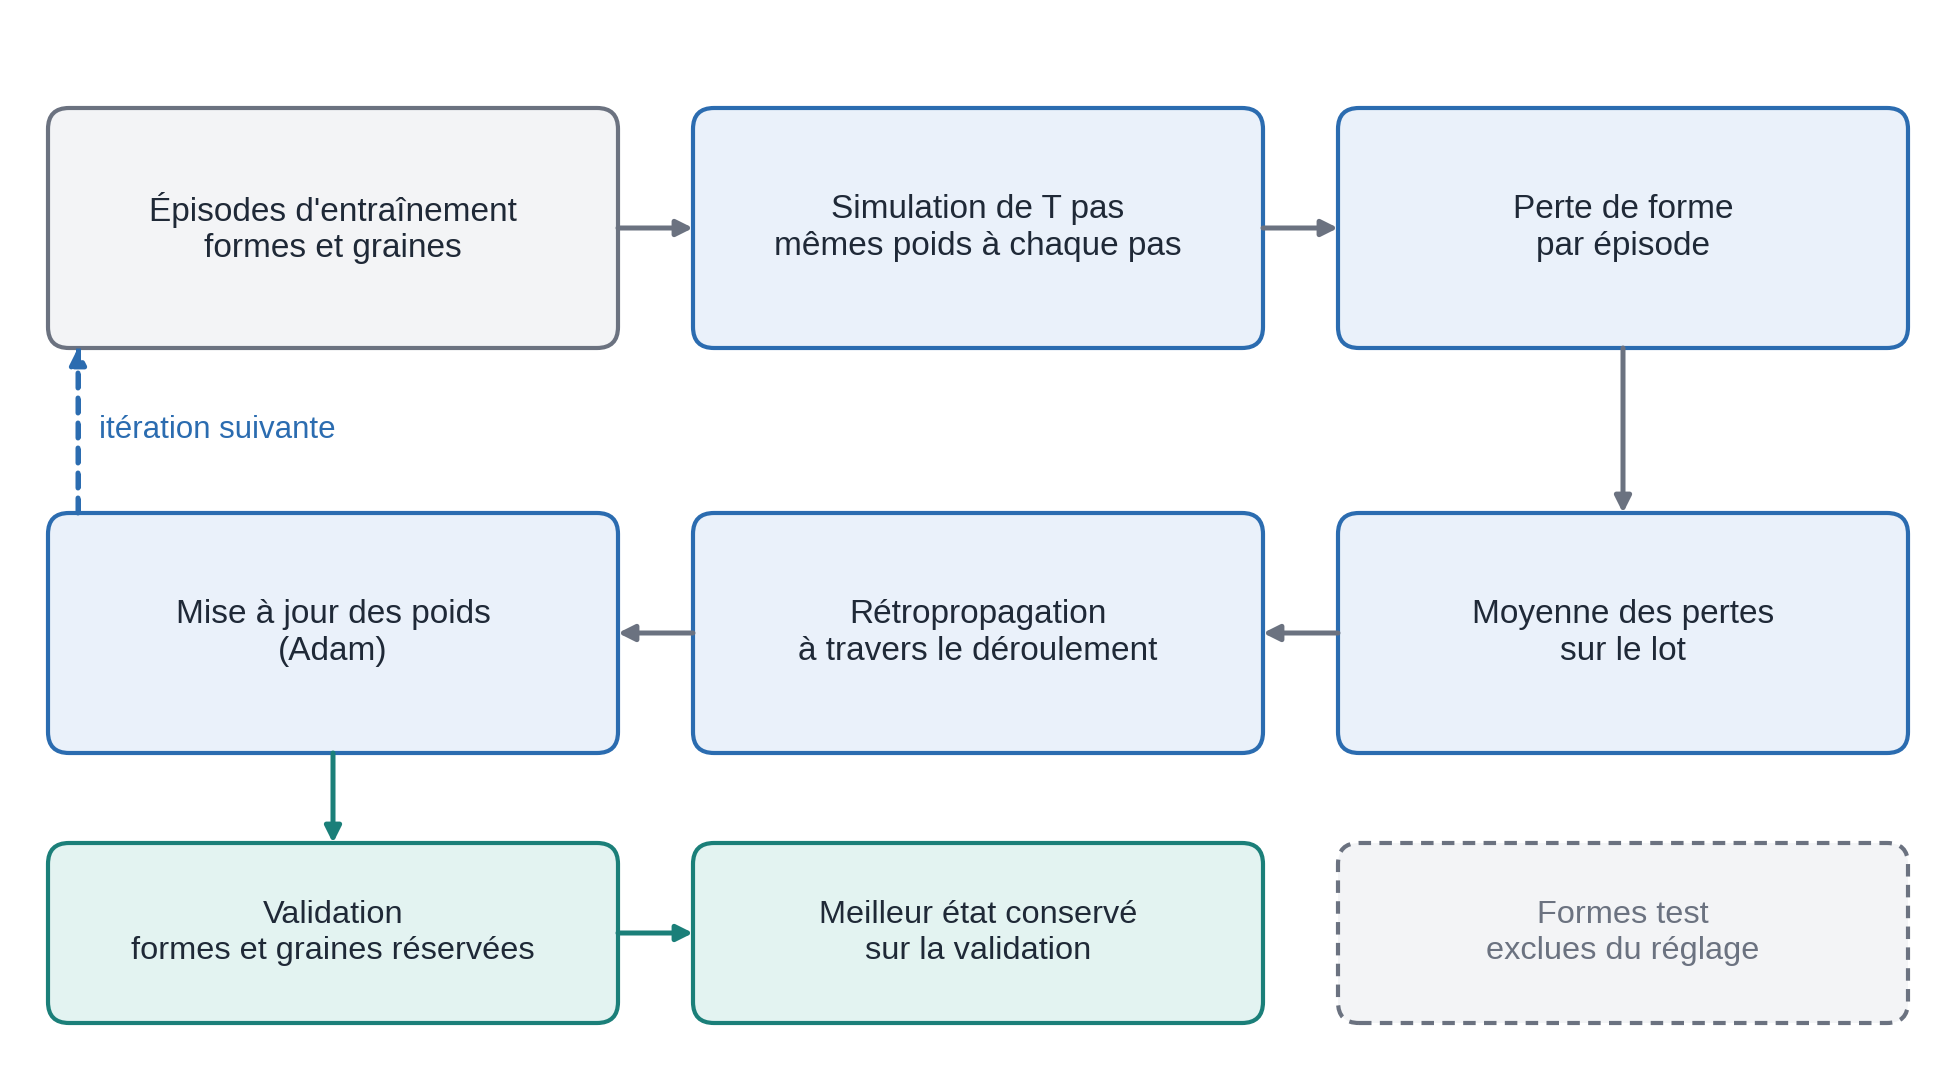
\includegraphics[width=0.46\textwidth,keepaspectratio]{images/differentiable_training_flow.png}\par
  \vspace{0.05cm}
  \begin{beamercolorbox}[wd=\textwidth,leftskip=0.4cm,dp=1.2em]{block body}
    \footnotesize\textbf{1 200 itérations · 8 épisodes par lot} --- Adam $0{,}001$, décroissance $0{,}999$, gradient borné à 1, validation toutes les 50 itérations, cinq graines prévues et une seule entraînée pour le GNN avec messages.
    \textit{Valeurs configurées, non des réglages optimaux : des hypothèses de travail, pas des résultats.}\par
  \end{beamercolorbox}
\end{frame}

% 10 --- Convention de succès
\begin{frame}{Le mot <<~succès~>> cache deux conventions}
  \begin{columns}[T]
    \begin{column}{0.5\textwidth}
      \textbf{\color{swarmblue}Convention actuelle}\\[0.2em]
      Un épisode réussit si, à partir d'un pas, \emph{toutes} les distances restent sous $0{,}15$ jusqu'à la fin.\par
      \textbf{\color{swarmblue}Convention historique} (celle du pilote)\\[0.2em]
      Premier franchissement de $0{,}5$ avant le dernier pas, sans exigence de maintien.\par
      \vspace{0.2em}
      {\footnotesize Un franchissement au seul dernier pas était exclu ; une distance finale sous le seuil pouvait rester un échec.\par}
    \end{column}
    \begin{column}{0.5\textwidth}
      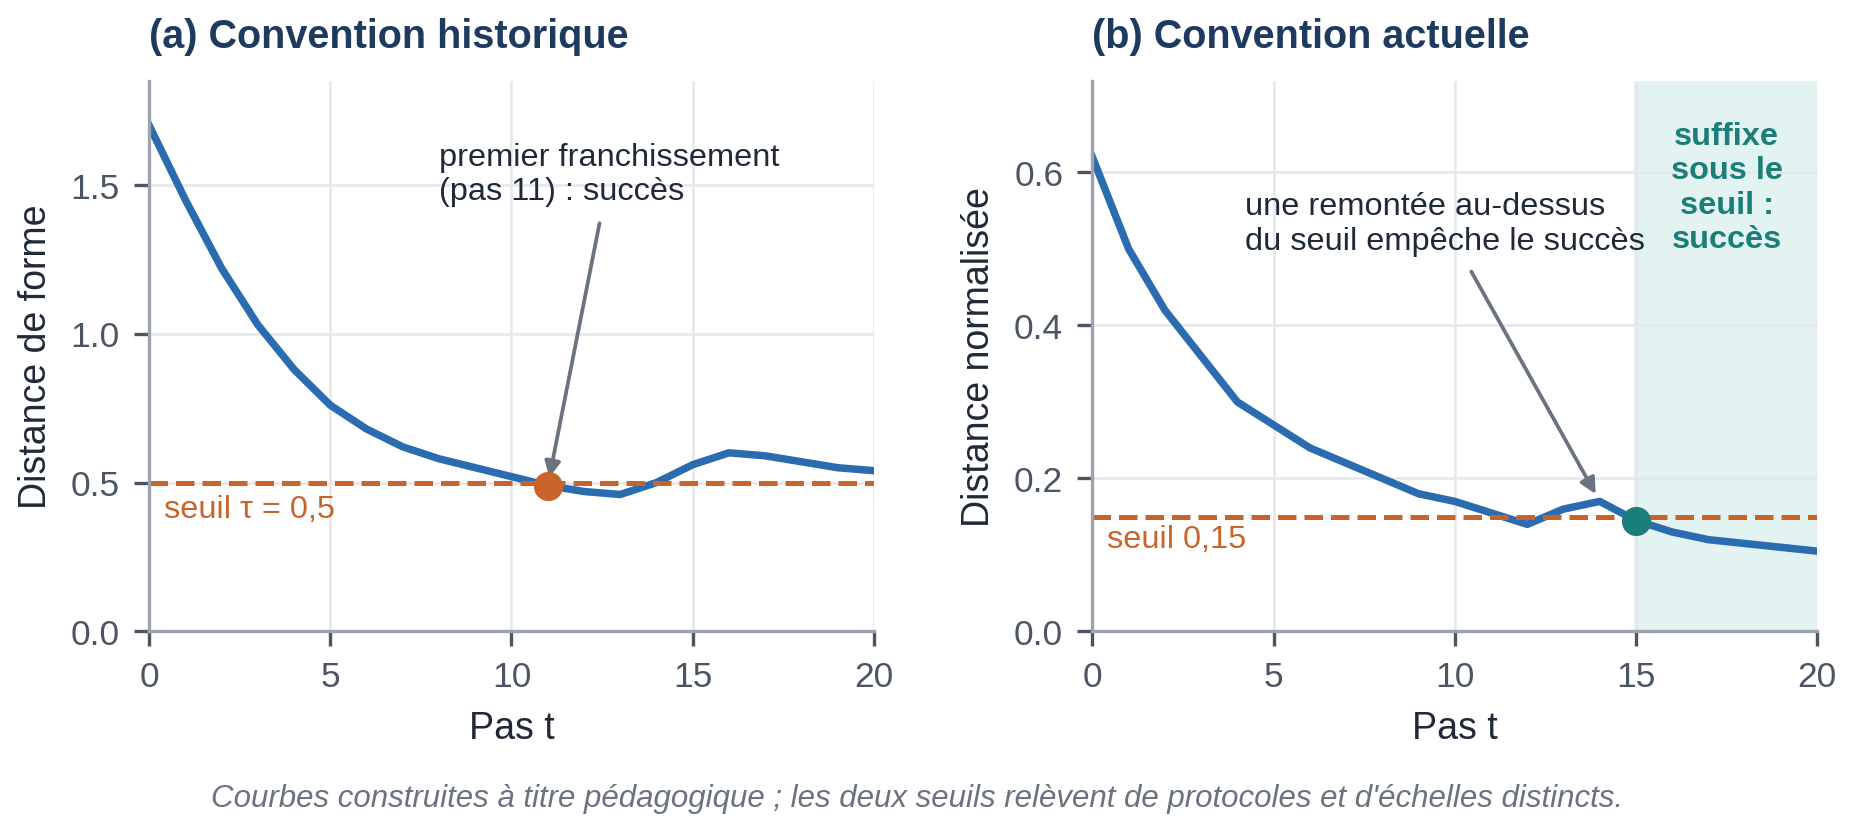
\includegraphics[width=\textwidth,keepaspectratio]{images/success_criterion_comparison.png}\par
      \vspace{0.15cm}
      {\footnotesize\itshape\color{swarmmuted} Même trajectoire, deux conventions : le pas rapporté et le verdict changent.\par}
    \end{column}
  \end{columns}
  \vspace{0.2cm}
  {\color{swarmblue}\textbf{Les deux ne donnent pas des pourcentages comparables} --- le pilote est lu avec ses propres seuils.\par}
\end{frame}

% 11 --- Passage à l'échelle
\begin{frame}{Passage à l'échelle : 20, 40 puis 100 robots}
  \begin{columns}[T]
    \begin{column}{0.5\textwidth}
      Distance de Chamfer moyenne, cible circulaire (rayon normalisé $=1$), pilote historique :\par
      \vspace{0.3em}
      \begin{tabular}{@{}lccc@{}}
        \toprule
        \textbf{Contrôleur} & \textbf{20} & \textbf{40} & \textbf{100} \\
        \midrule
        GNN (appris)        & 0,592 & 0,522 & 0,428 \\
        Regroupement (écrit)& 3,956 & 3,799 & 3,507 \\
        \midrule
        Succès rapporté     & 10\%  & 30\%  & 100\% \\
        \bottomrule
      \end{tabular}
      \vspace{0.5em}
      {\footnotesize\color{swarmmuted} Une valeur de succès très dépendante du seuil.\par}
    \end{column}
    \begin{column}{0.5\textwidth}
      \begin{itemize}\footnotesize
        \item Dix épisodes par condition, pilote historique : le modèle évalué vient du curriculum réduit, pas de l'implémentation actuelle.
        \item La même politique s'exécute à 40 et 100 robots sans changer un seul poids : propriété structurelle, à mesurer quand même.
        \item Le regroupement ne reçoit pas la consigne de cercle : l'écart mesure aussi une asymétrie d'information.
        \item La baisse peut venir de la densité de robots sur le contour, pas de la seule qualité de la politique.
        \item Une distance plus faible ne prouve ni une forme lisible, ni une robustesse générale.
      \end{itemize}
    \end{column}
  \end{columns}
\end{frame}

% 12 --- Robustesse
\begin{frame}{Pannes simulées et dispersion entre graines}
  \begin{columns}[T]
    \begin{column}{0.46\textwidth}
      \begin{itemize}\footnotesize
        \item Retraits de 5, 10 puis 20\,\% des robots à mi-épisode : $0{,}592 \to 0{,}638$, soit $+8\,\%$ de distance moyenne.
        \item Un robot retiré est figé, ses commandes sont annulées : déconnexion propre.
        \item Le regroupement varie du même ordre en absolu, à un niveau six fois plus élevé.
        \item Entre graines, la distance finale varie d'environ 47\,\% ; un seul épisode sur dix franchit le seuil avant le dernier pas.
        \item Dix épisodes par condition : aucun intervalle de confiance exploitable.
      \end{itemize}
    \end{column}
    \begin{column}{0.54\textwidth}
      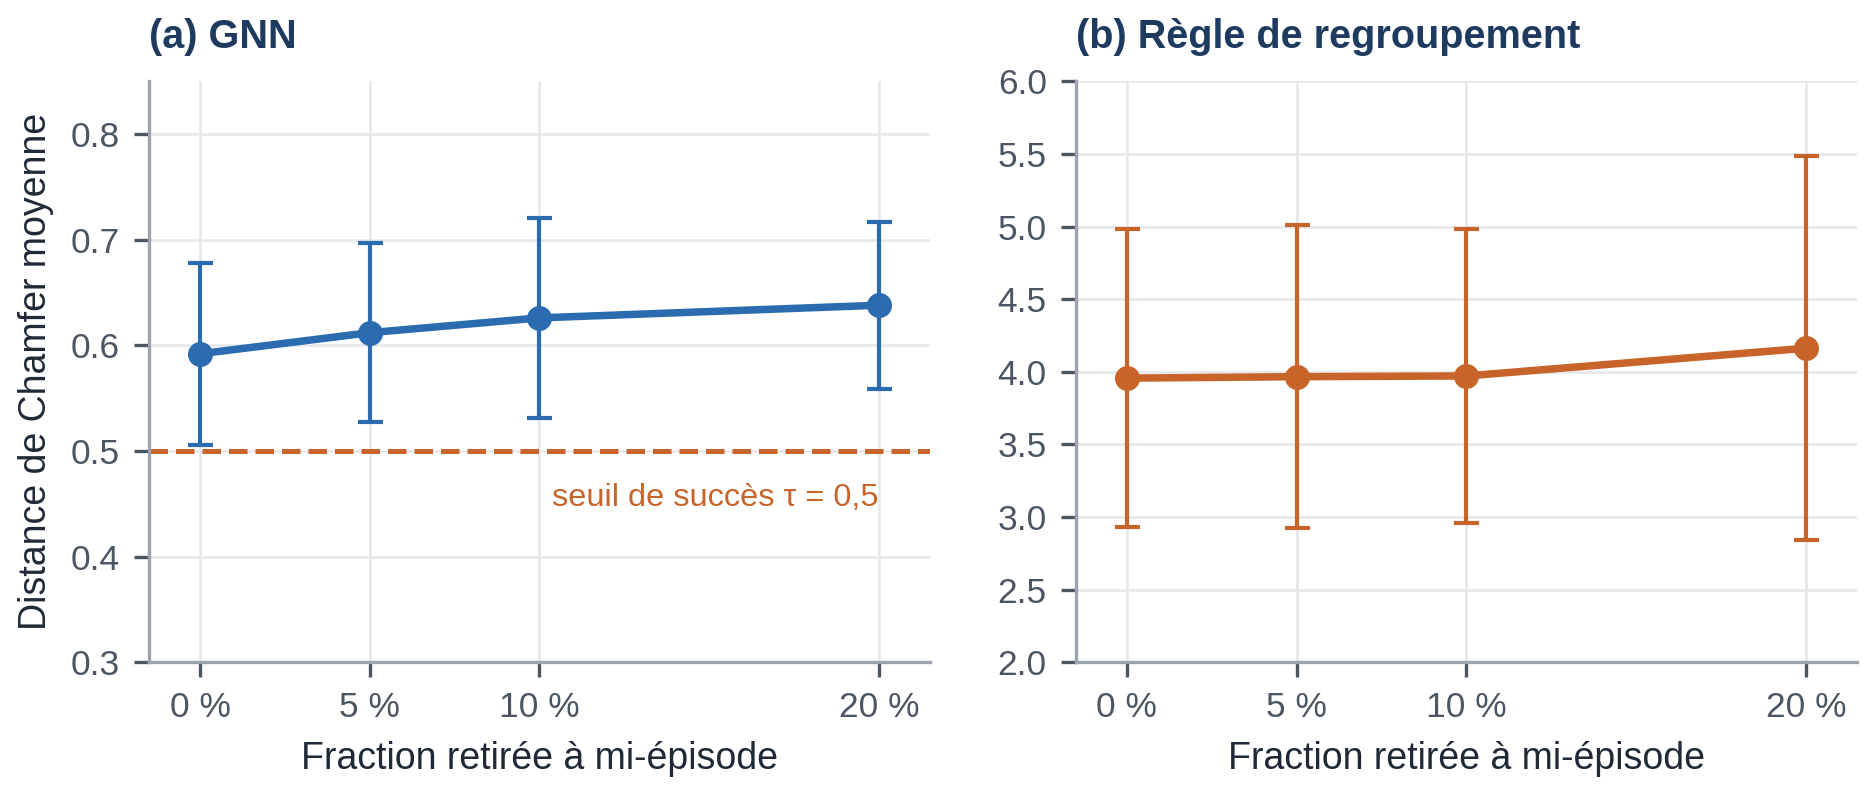
\includegraphics[width=0.92\textwidth,keepaspectratio]{images/historical_chamfer_vs_failures.png}\par
      \vspace{0.05cm}
      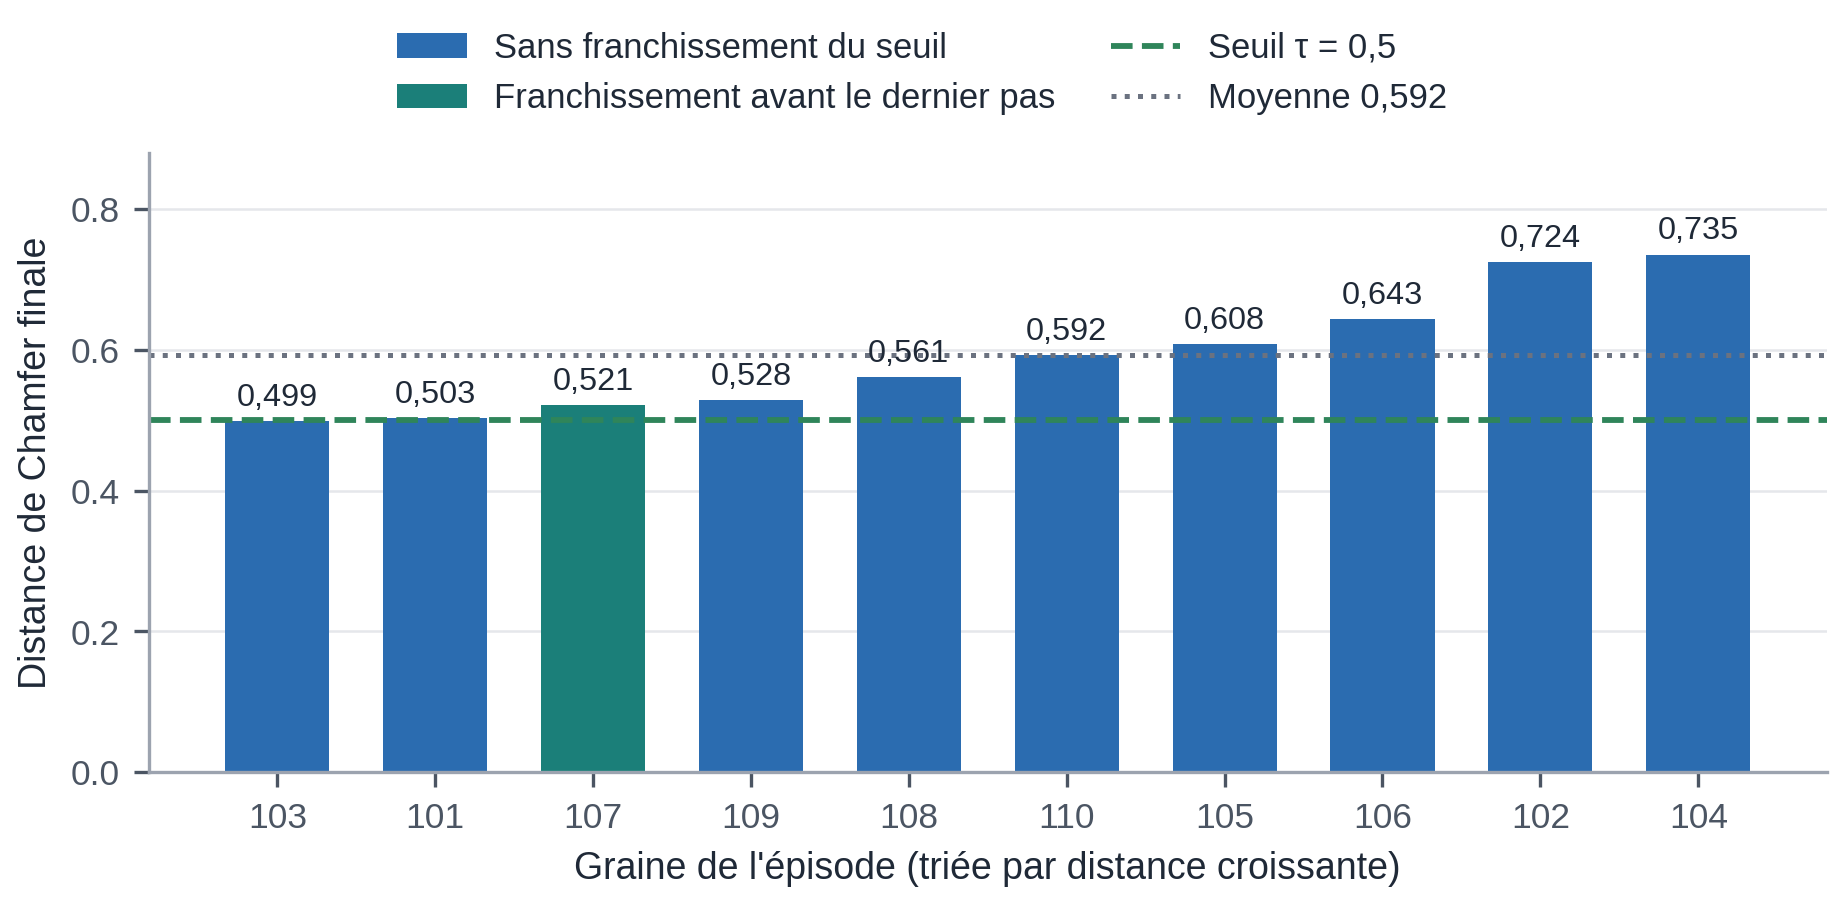
\includegraphics[width=0.92\textwidth,keepaspectratio]{images/historical_seed_dispersion.png}\par
      \vspace{0.05cm}
      {\scriptsize\itshape\color{swarmmuted} À gauche : distance selon la fraction retirée. À droite : dix graines, 20 robots sans retrait.\par}
    \end{column}
  \end{columns}
\end{frame}

% 13 --- Curriculum
\begin{frame}{Curriculum réduit : où s'arrête la preuve}
  \begin{columns}[T]
    \begin{column}{0.5\textwidth}
      \textbf{\color{swarmblue}Quatre étapes cumulatives, sans accès au test}\\
      {\footnotesize 3, puis 6, puis 9, puis 11 cibles ; chaque niveau reprend les cibles précédentes.\par}
      \vspace{0.4em}
      \textbf{\color{swarmblue}Perte en fin d'étape : $0{,}362$, puis $0{,}251$, $0{,}240$, $0{,}117$}\\
      {\footnotesize\color{swarmmuted} Ces quatre nombres ne sont pas comparables : le jeu de cibles change à chaque étape.\par}
      \vspace{0.4em}
      \textbf{\color{swarmblue}Le seul signal lisible : les cibles anciennes}\\
      {\footnotesize Sur les cibles vues depuis le début, la perte descend de $0{,}333$ à $0{,}216$ puis $0{,}163$.\par}
      \vspace{0.4em}
      \textbf{\color{swarmblue}Portée réelle}\\
      {\footnotesize Une graine, un budget réduit, des cibles uniquement symboliques (A, B, C, 010, 123) : un résultat de faisabilité, pas une mesure de capacité.\par}
    \end{column}
    \begin{column}{0.5\textwidth}
      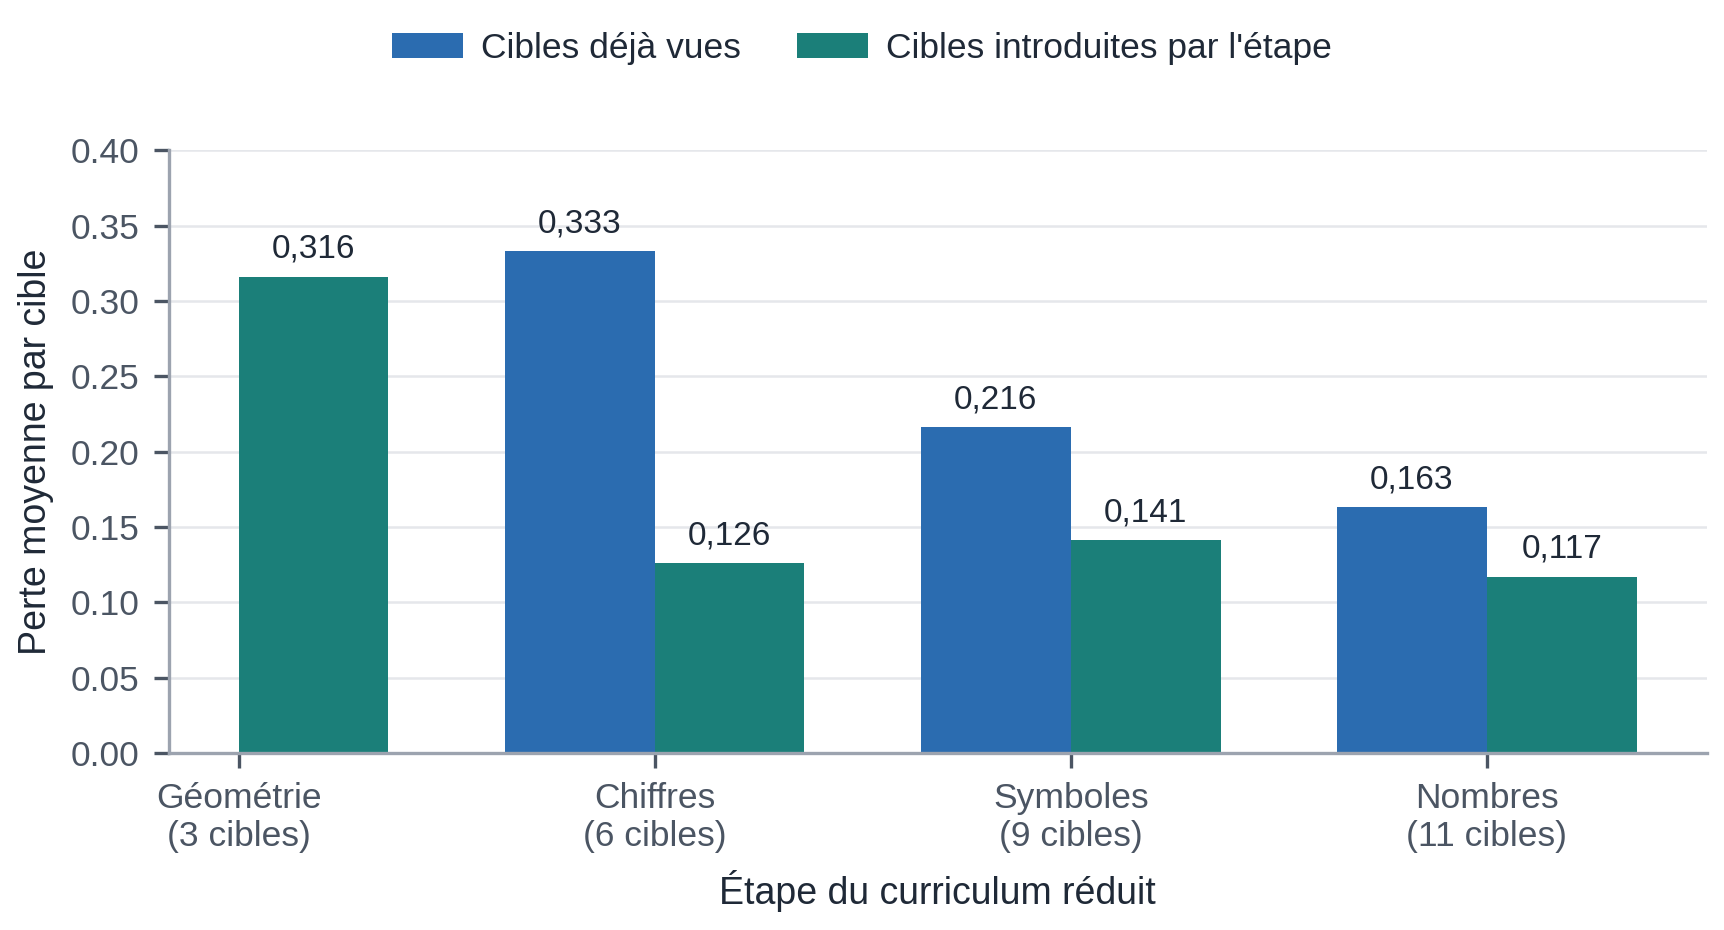
\includegraphics[width=0.9\textwidth,keepaspectratio]{images/historical_curriculum_per_target.png}\par
      \vspace{0.1cm}
      {\footnotesize\itshape\color{swarmmuted} Perte par cible au fil des quatre étapes (pilote historique).\par}
      \vspace{0.3em}
      \begin{block}{À retenir}
        \footnotesize Le curriculum a fonctionné : les formes anciennes restent atteintes. Pas de preuve d'un apprentissage plus rapide. La campagne prévue ajoutera cinq graines d'entraînement, cinquante répétitions par condition et des cibles tenues hors entraînement avant la mesure.
      \end{block}
    \end{column}
  \end{columns}
\end{frame}

% 14 --- Menaces à la validité
\begin{frame}{Menaces à la validité : ce qui n'est pas revendiqué}
  \begin{columns}[T]
    \begin{column}{0.46\textwidth}
      \textbf{\color{swarmblue}Validité interne}\\
      {\footnotesize Dix épisodes par condition, une seule graine pilotée. Le couplage curriculum / architecture n'est pas séparé. La variante sans communication est entraînée et évaluée : c'est son analyse qui manque, le GNN avec messages n'ayant qu'un seul run.\par}
      \vspace{0.4em}
      \textbf{\color{swarmblue}Validité externe}\\
      {\footnotesize Repère commun, positions exactes sans capteur bruité, aucun délai ni perte de message, panne propre, arène finie ; vingt pas d'horizon au pilote, 40 à l'entraînement et 120 à l'évaluation depuis.\par}
      \vspace{0.4em}
      \textbf{\color{swarmblue}Ce que la mesure ne dit pas}\\
      {\footnotesize La distance de forme est aveugle à la lisibilité de la figure ; le seuil de succès est un choix opérationnel ; un taux de collisions n'est pas un impact mécanique.\par}
    \end{column}
    \begin{column}{0.54\textwidth}
      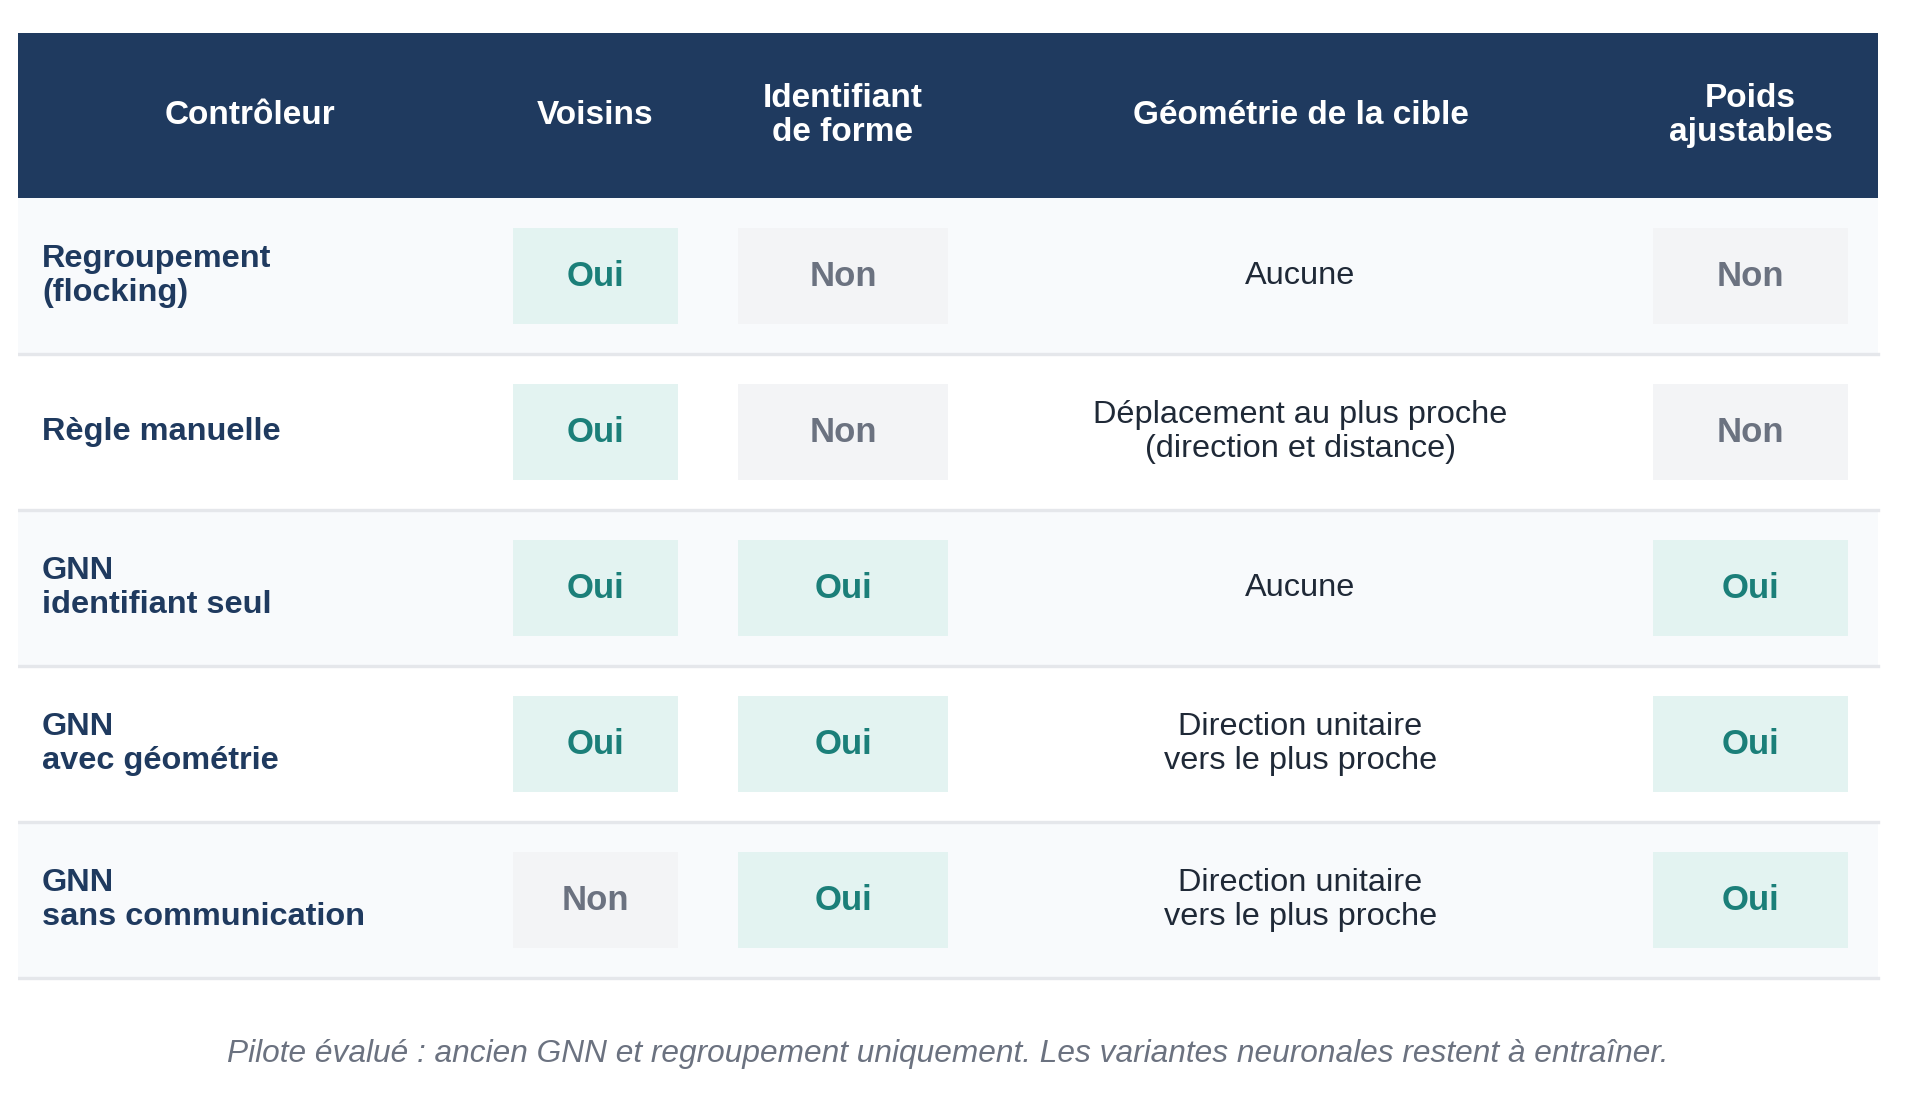
\includegraphics[width=\textwidth,keepaspectratio]{images/controller_information_matrix.png}\par
      \vspace{0.15cm}
      {\footnotesize\itshape\color{swarmmuted} Ce que chaque contrôleur reçoit à l'exécution : voisinage, identifiant de forme, géométrie cible, poids ajustables. Cette matrice décrit ce qui est préparé, pas des performances : le pilote n'a évalué que l'ancien GNN et le regroupement.\par}
    \end{column}
  \end{columns}
  \vspace{0.2em}
  {\color{swarmblue}\textbf{Ce que le mémoire revendique :} une chaîne complète et vérifiable, des instruments prêts à l'emploi, et un pilote dont l'échec est expliqué puis corrigé.\par}
\end{frame}

% 15 --- Conclusion
{
\setbeamercolor{background canvas}{bg=swarmnavy}
\setbeamercolor{normal text}{fg=white, bg=swarmnavy}
\setbeamercolor{frametitle}{fg=white, bg=swarmnavy}
\setbeamercolor{itemize item}{fg=swarmgold}
\begin{frame}{Bilan : ce qui est établi, ce qui reste à conduire}
  \color{white}\relax
  \begin{columns}[T]
    \begin{column}{0.5\textwidth}
      \textbf{\color{swarmgold}CE QUI EST ÉTABLI}
      \begin{itemize}\footnotesize\color{white}
        \item Une commande décentralisée, sans coordinateur ni identifiant de forme global.
        \item Un apprentissage différentiable sur simulation complète, sélectionné sur validation.
        \item Une chaîne d'évaluation, de robustesse et de lisibilité prête à l'emploi.
        \item Un pilote dont l'échec est diagnostiqué : décroissance du pas trop rapide et politique gelée.
        \item Correctifs appliqués et vérifiés sur un run court.
      \end{itemize}
    \end{column}
    \begin{column}{0.5\textwidth}
      \textbf{\color{swarmgold}CE QUI RESTE À CONDUIRE}
      \begin{itemize}\footnotesize\color{white}
        \item Au moins 50 départs par condition et cinq graines d'entraînement.
        \item Analyser les variantes déjà entraînées : la même consigne, sans message, et la règle manuelle à consigne comparable.
        \item Bruit d'observation, suppression d'arêtes, portée réduite.
        \item Un questionnaire aveugle sur la lisibilité des figures.
        \item Aucun résultat d'entraînement accepté pour l'implémentation actuelle.
      \end{itemize}
    \end{column}
  \end{columns}
  \vfill
  \begin{center}
    {\color{white}\LARGE\bfseries Merci de votre attention\par}
    \vspace{0.4em}
    {\color{swarmgold}\rule{2.4cm}{1.2pt}\par}
    \vspace{0.5em}
    {\footnotesize Laurent MWANAMPUTU LABEYA --- Soutenance de mémoire, UNIKIN\par}
  \end{center}
\end{frame}
}

\end{document}
